% PREAMBLE
\documentclass[11pt]{amsart}
\usepackage[T1]{fontenc}
\usepackage{lmodern}
\usepackage{microtype}
\usepackage{amsmath,amssymb}
\usepackage{mathtools}
\usepackage{graphicx}
\usepackage{booktabs}
\usepackage{tikz}
\usepackage[colorlinks=true,linkcolor=blue!45!black,citecolor=blue!45!black,urlcolor=blue!45!black]{hyperref}
\usepackage[capitalize]{cleveref}

\newtheorem{theorem}{Theorem}[section]
\newtheorem{proposition}[theorem]{Proposition}
\newtheorem{lemma}[theorem]{Lemma}
\newtheorem{corollary}[theorem]{Corollary}
\newtheorem{conjecture}[theorem]{Conjecture}
\theoremstyle{definition}
\newtheorem{definition}[theorem]{Definition}
\newtheorem{fact}[theorem]{Fact}
\theoremstyle{remark}
\newtheorem{remark}[theorem]{Remark}

\definecolor{polyg}{HTML}{4059AD}
\definecolor{centd}{HTML}{6B4FA0}

\title{The Sequence Census of a Parity Design}
\author{Carlo Mitchener}
\email{carlo.mitchener@gmail.com}
\date{2026-08-31}

% PAPER
\begin{document}

\begin{abstract}
A single odd-or-even rule on the corners of a cube grows a fractal, and every way of counting that fractal writes down an integer sequence. This paper counts the sequences. In dimension $D$ the rules number $2^{2^{D}}$, but between them they write only $\prod_{w=0}^{D}\bigl(1+\binom{D}{w}\bigr)$ distinct sequences as the grid grows, every nonempty one a polynomial of degree $D$; as the fractal deepens instead, the cell and void counts are C-finite of order at most two and the exposed-face counts of order at most $D+1$, on roots read off the tile. In the plane the census is completely classical: every nonzero fill sequence is a polygonal number, a centered polygonal number, one of those read at a reflected argument, or a multiple of the oblong numbers, and which of them is decided by two bits of the rule and the number of corners it keeps. The polygonal numbers that keep appearing here therefore arrive by one mechanism and not by coincidence; and where a genuinely different mechanism lands on the same family, that collision is forced, since a quadratic normalised at $0$ and $1$ is pinned by its leading coefficient alone.
\end{abstract}

\maketitle

\section{Introduction}
\label{sec:intro}

Colour the cells of a square grid by the parity of their two coordinates, choose which of the four colours to keep, and count what you kept. There are sixteen choices. Keep only the cells with both coordinates even and you count $1, 4, 9, 16, \dots$, the squares. Keep the cells with at most one odd coordinate and you count $1, 8, 21, 40, \dots$, the octagonal numbers. Keep the cells whose coordinates have the same parity and you count $1, 5, 13, 25, \dots$, the centered squares. All six rules that behave this way are drawn in \cref{fig:families}.

\begin{figure}[!ht]
\centering
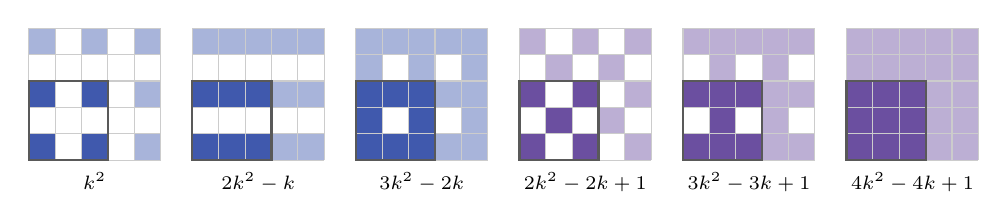
\begin{tikzpicture}[scale=0.335,capt/.style={anchor=north,inner sep=1pt}]
\begin{scope}[shift={(0.0,0)}]
  \foreach \i in {0,2,4} \foreach \j in {0,2,4} {\fill[polyg] (\i,\j) rectangle ++(1,1);}
  \fill[white,opacity=0.55] (3,0) rectangle (5,5);
  \fill[white,opacity=0.55] (0,3) rectangle (3,5);
  \draw[step=1,gray!40] (0,0) grid (5,5);
  \draw[black!65,thick] (0,0) rectangle (3,3);
  \node[capt] at (2.5,-0.35) {\scriptsize $k^{2}$};
\end{scope}
\begin{scope}[shift={(6.2,0)}]
  \foreach \i in {0,...,4} \foreach \j in {0,2,4} {\fill[polyg] (\i,\j) rectangle ++(1,1);}
  \fill[white,opacity=0.55] (3,0) rectangle (5,5);
  \fill[white,opacity=0.55] (0,3) rectangle (3,5);
  \draw[step=1,gray!40] (0,0) grid (5,5);
  \draw[black!65,thick] (0,0) rectangle (3,3);
  \node[capt] at (2.5,-0.35) {\scriptsize $2k^{2}-k$};
\end{scope}
\begin{scope}[shift={(12.4,0)}]
  \foreach \i in {0,...,4} \foreach \j in {0,2,4} {\fill[polyg] (\i,\j) rectangle ++(1,1);}
  \foreach \i in {0,2,4} \foreach \j in {1,3} {\fill[polyg] (\i,\j) rectangle ++(1,1);}
  \fill[white,opacity=0.55] (3,0) rectangle (5,5);
  \fill[white,opacity=0.55] (0,3) rectangle (3,5);
  \draw[step=1,gray!40] (0,0) grid (5,5);
  \draw[black!65,thick] (0,0) rectangle (3,3);
  \node[capt] at (2.5,-0.35) {\scriptsize $3k^{2}-2k$};
\end{scope}
\begin{scope}[shift={(18.6,0)}]
  \foreach \i in {0,2,4} \foreach \j in {0,2,4} {\fill[centd] (\i,\j) rectangle ++(1,1);}
  \foreach \i in {1,3} \foreach \j in {1,3} {\fill[centd] (\i,\j) rectangle ++(1,1);}
  \fill[white,opacity=0.55] (3,0) rectangle (5,5);
  \fill[white,opacity=0.55] (0,3) rectangle (3,5);
  \draw[step=1,gray!40] (0,0) grid (5,5);
  \draw[black!65,thick] (0,0) rectangle (3,3);
  \node[capt] at (2.5,-0.35) {\scriptsize $2k^{2}-2k+1$};
\end{scope}
\begin{scope}[shift={(24.8,0)}]
  \foreach \i in {0,...,4} \foreach \j in {0,2,4} {\fill[centd] (\i,\j) rectangle ++(1,1);}
  \foreach \i in {1,3} \foreach \j in {1,3} {\fill[centd] (\i,\j) rectangle ++(1,1);}
  \fill[white,opacity=0.55] (3,0) rectangle (5,5);
  \fill[white,opacity=0.55] (0,3) rectangle (3,5);
  \draw[step=1,gray!40] (0,0) grid (5,5);
  \draw[black!65,thick] (0,0) rectangle (3,3);
  \node[capt] at (2.5,-0.35) {\scriptsize $3k^{2}-3k+1$};
\end{scope}
\begin{scope}[shift={(31.0,0)}]
  \foreach \i in {0,...,4} \foreach \j in {0,...,4} {\fill[centd] (\i,\j) rectangle ++(1,1);}
  \fill[white,opacity=0.55] (3,0) rectangle (5,5);
  \fill[white,opacity=0.55] (0,3) rectangle (3,5);
  \draw[step=1,gray!40] (0,0) grid (5,5);
  \draw[black!65,thick] (0,0) rectangle (3,3);
  \node[capt] at (2.5,-0.35) {\scriptsize $4k^{2}-4k+1$};
\end{scope}
\end{tikzpicture}
\caption{The six rules of the plane that keep the all-even corner, at side $n = 2k-1 = 5$: codes $1, 3, 7$ drop the cells with both coordinates odd and count polygonal numbers, codes $9, 11, 15$ keep them and count centered polygonal numbers (\cref{thm:plane}). The heavy square is the previous size $k = 2$.}
\label{fig:families}
\end{figure}

Three classical families out of three tries is either a mechanism or a coincidence, and the first purpose of this paper is to decide which. The answer is a mechanism, and a complete one: in the plane \emph{every} such count is a classical figurate number, and which family it belongs to is read off the rule by inspection (\cref{thm:plane}). For the six rules that keep the all-even corner -- the three above among them -- the reading is exactly a polygonal or a centered polygonal number.

The rule generalises. Fix a dimension $D$; a \emph{design} is a subset $F$ of the parity cube $\{0,1\}^{D}$, and a cell of a $D$-dimensional grid is filled when the parities of its coordinates spell a corner of $F$. Substituting the rule into itself by the Kronecker product turns a design into a fractal -- the Sierpi\'nski carpet is the two-dimensional rule that drops the all-odd corner, the Menger sponge the three-dimensional rule that keeps the corners of weight at most one -- so a design is a compact name for a fractal, and the counting sequences of that fractal are what this paper enumerates.

There are four ways to let such a picture grow, and each writes sequences of a different kind.

\begin{itemize}
\item The \emph{side axis}: hold the rule, grow the grid to odd side $n = 2k-1$, count the filled cells as $k$ runs. This writes a polynomial, of degree $D$ for every nonempty rule (\cref{thm:fill}).
\item The \emph{level axis}: hold the tile at a fixed odd side, substitute it into itself $L$ times, count cells, voids or exposed faces as $L$ runs. This writes C-finite sequences: order at most two for cells and voids, at most $D+1$ for exposed faces, with roots read off the tile (\cref{prop:level,thm:surface}).
\item The \emph{symmetry axis}: count the designs themselves, up to the symmetries of the cube, as $D$ grows. This writes a Burnside average, and it is not C-finite (\cref{prop:notcfinite}).
\item The \emph{arithmetic axis}: count the filled cells that are visible from the origin. This is not C-finite either, and for one such sequence that is a theorem \cite{coprimepaper}.
\end{itemize}

The census question -- how many sequences, not which -- has a clean answer on the side axis. The $2^{2^{D}}$ designs of dimension $D$ write only $\prod_{w=0}^{D}\bigl(1+\binom{D}{w}\bigr)$ distinct sequences between them (\cref{cor:census}), because the fill polynomial remembers only how many kept corners carry each Hamming weight. Set beside the number of designs \emph{up to cube symmetry}, that count tells a story with a crossing in it: in dimensions one through four a design has more distinct sequences available to it than distinct shapes, and from dimension five onwards the shapes outnumber the sequences without bound (\cref{thm:crossover}). The machine draws far more pictures than it can count.

\subsection*{What is and is not new here}

The fill of a design is an Ehrhart-type count -- lattice points of a dilated box lying in prescribed cosets of $(2\mathbb{Z})^{D}$ -- and quasi-polynomiality is standard \cite{beckrobins}; restricted to odd sides the count is an honest polynomial and \cref{thm:fill} is a two-line special case, not an application of the general theory. The polygonal and centered polygonal numbers are classical, and no novelty is claimed for them or for the individual catalogue entries they carry. Burnside's lemma is classical \cite{rotman}. The recurrence order of the diagonal slice census is a companion paper's theorem \cite{slicepaper}, the coprimality density and the failure of C-finiteness for the visible-point count are another's \cite{coprimepaper}, and the classification of designs whose fill is a divisor count is a third's \cite{avatarpaper}.

What is offered here is the census itself: the count of distinct fill sequences (\cref{cor:census}), the two-bit reading of the plane that turns six catalogue collisions into one theorem (\cref{thm:plane}) together with its shell law (\cref{prop:shell}), the endpoint and mirror laws that drive it (\cref{prop:endpoints,prop:mirror}), the surface law in the generality that covers every design rather than the symmetric ones (\cref{thm:surface}), the crossover between the two censuses (\cref{thm:crossover}), the observation that the classical families are a bottleneck rather than a signal (\cref{prop:pigeon}), and the exact accounting of which of these sequences the catalogue already holds.

\Cref{sec:def} fixes the objects. \Cref{sec:res} states everything, axis by axis. \Cref{sec:proofs} proves it. \Cref{sec:repro} names the script, its domain and its runtime.

\section{Definitions}
\label{sec:def}

Throughout $D \ge 1$ is an integer and $k \ge 1$ an integer parameter. Sequence identifiers of the form A\textit{nnnnnn} refer to entries of the On-Line Encyclopedia of Integer Sequences \cite{oeis}.

\begin{definition}[design, weight signature, code]
\label{def:design}
The \emph{parity cube} is $\{0,1\}^{D}$; its elements are \emph{corners} and the \emph{weight} of a corner $c$ is $|c| = c_{1}+\cdots+c_{D}$. A \emph{design} is a subset $F \subseteq \{0,1\}^{D}$. Its \emph{weight signature} is $f = (f_{0},\dots,f_{D})$ with $f_{w} = \#\{c \in F : |c| = w\}$, and its \emph{popcount} is $|F| = \sum_{w}f_{w}$. Its \emph{code} is $\sum_{c \in F}2^{\,c_{1}+2c_{2}+\cdots+2^{D-1}c_{D}}$, an integer below $2^{2^{D}}$ that names the design uniquely.
\end{definition}

\begin{definition}[fill]
\label{def:fill}
Let $B_{k} = \{0,1,\dots,2k-2\}^{D}$ be the cubical grid of odd side $n = 2k-1$. The \emph{parity} of a cell $x \in B_{k}$ is the corner $\pi(x)$ with $\pi(x)_{i} = x_{i} \bmod 2$. A cell is \emph{filled} by $F$ when $\pi(x) \in F$, and the \emph{fill} of $F$ is
\[
  P_{F}(k) = \#\{\,x \in B_{k} : \pi(x) \in F\,\}.
\]
The \emph{void} count is $V_{F}(k) = (2k-1)^{D} - P_{F}(k)$. A coordinate of $B_{k}$ takes $k$ even values and $k-1$ odd ones, which is why $k$ and not $n$ is the natural variable.
\end{definition}

\begin{definition}[tile, fractal, level]
\label{def:level}
For odd $q = 2k-1$ the \emph{tile} of $F$ is the filled subset of $\{0,\dots,q-1\}^{D}$, of size $P_{F}(k)$. The \emph{fractal at level $L$} is the $L$-fold Kronecker substitution of the tile into itself: a cell of $\{0,\dots,q^{L}-1\}^{D}$ is filled when every one of its $L$ base-$q$ digit vectors lies in the tile. Write $\mathrm{cell}_{F}(L)$ for its cell count and $\mathrm{sur}_{F}(L)$ for the number of unit $(D-1)$-faces lying in exactly one filled cell.
\end{definition}

\begin{definition}[cube symmetry]
\label{def:sym}
The \emph{cube group} $B_{D}$ acts on corners by $c \mapsto (c_{\sigma(1)} \oplus t_{1},\dots,c_{\sigma(D)} \oplus t_{D})$ for a permutation $\sigma$ of the axes and a vector $t \in \{0,1\}^{D}$; it has order $2^{D}D!$. Two designs are the same \emph{shape} when they lie in one $B_{D}$-orbit.
\end{definition}

\begin{definition}[the classical families]
\label{def:classical}
For $m \ge 3$ the $m$-gonal numbers and the centered $m$-gonal numbers are
\[
  P_{m}(k) = \frac{(m-2)k^{2}-(m-4)k}{2},
  \qquad
  C_{m}(k) = \frac{m\,k(k-1)}{2}+1 .
\]
Thus $P_{4},P_{6},P_{8}$ are the squares, hexagonal and octagonal numbers A000290, A000384, A000567, and $C_{4},C_{6},C_{8}$ are the centered squares, centered hexagonal numbers and odd squares A001844, A003215, A016754.
\end{definition}

\begin{definition}[C-finite]
\label{def:cfinite}
A sequence $a$ is \emph{C-finite} of order $r$ when $a(n) = \sum_{i=1}^{r}\lambda_{i}a(n-i)$ for all large $n$, with the $\lambda_{i}$ constants independent of $n$.
\end{definition}

\section{Results}
\label{sec:res}

\subsection*{The side axis writes polynomials, and the polynomial remembers only the signature}

\begin{theorem}[fill law]
\label{thm:fill}
For every design $F$ of dimension $D$ and every $k \ge 1$,
\[
  P_{F}(k) \;=\; \sum_{c \in F} k^{\,D-|c|}(k-1)^{|c|} \;=\; \sum_{w=0}^{D} f_{w}\,k^{\,D-w}(k-1)^{w}.
\]
This agrees with a polynomial in $k$ of degree exactly $D$ and leading coefficient $|F|$ when $F \neq \emptyset$, and with the zero polynomial otherwise.
\end{theorem}

\begin{lemma}[the fill basis is a basis]
\label{lem:basis}
The $D+1$ polynomials $q_{w}(k) = k^{D-w}(k-1)^{w}$, $w = 0,\dots,D$, are linearly independent over $\mathbb{Q}$. Consequently $P_{F}$ determines the weight signature $f$ outright.
\end{lemma}

\begin{corollary}[the sequence census of the side axis]
\label{cor:census}
The number of distinct sequences $P_{F}$, over all $2^{2^{D}}$ designs of dimension $D$, is exactly
\[
  N(D) \;=\; \prod_{w=0}^{D}\Bigl(1+\binom{D}{w}\Bigr),
\]
which is A129824 at index $D$: $2$, $4$, $12$, $64$, $700$, $17424$, $1053696$, $160579584$, $62856336636$ for $D = 0,\dots,8$.
\end{corollary}

\begin{proposition}[endpoint law]
\label{prop:endpoints}
$P_{F}(1) = f_{0}$ and $P_{F}(0) = (-1)^{D}f_{D}$. So the value at $k=1$ reports whether the design keeps the all-even corner -- equivalently whether the single cell of the grid of side one is filled -- and the value at $k=0$ reports, up to sign, whether it keeps the all-odd corner.
\end{proposition}

\begin{proposition}[mirror law]
\label{prop:mirror}
Let $F^{\ast}$ be any design whose weight signature is $f$ reversed. Then $P_{F^{\ast}}(k) = (-1)^{D}P_{F}(1-k)$ as polynomials. Moreover the $D$-th finite difference of $P_{F}$ is the constant $D!\,|F|$.
\end{proposition}

\subsection*{The plane, completely}

\begin{theorem}[the plane is classical]
\label{thm:plane}
Let $D = 2$, let $F$ be a nonempty design with signature $(f_{0},f_{1},f_{2})$ and popcount $p = |F|$.
\begin{enumerate}
\item[(i)] If $f_{0}=1$ and $f_{2}=0$ then $P_{F} = P_{2p+2}$, the $(2p+2)$-gonal number. The three cases $p = 1,2,3$ are the squares, the hexagonal numbers and the octagonal numbers.
\item[(ii)] If $f_{0}=1$ and $f_{2}=1$ then $P_{F} = C_{2p}$, the centered $2p$-gonal number. The three cases $p = 2,3,4$ are the centered squares, the centered hexagonal numbers and the odd squares.
\item[(iii)] If $f_{0}=0$ and $f_{2}=1$ then $P_{F}(k) = P_{2p+2}(1-k)$: the same polygonal number as in (i), read at the reflected argument.
\item[(iv)] If $f_{0}=f_{2}=0$ then $P_{F}(k) = f_{1}\,k(k-1) = 2f_{1}T_{k-1}$, a multiple of the oblong numbers, with $T_{j}$ the $j$-th triangular number.
\end{enumerate}
So each of the eleven nonzero fill sequences of the plane is classical: three are polygonal numbers, three centered polygonal numbers, three polygonal numbers at a reflected argument, and two are oblong multiples. The branch is decided by two bits of the rule and the number of sides by the popcount alone.
\end{theorem}

\begin{proposition}[shell law]
\label{prop:shell}
For $D = 2$ and every $k$,
\[
  P_{F}(k)-P_{F}(k-1) \;=\; 2|F|\,(k-1) + f_{0} - f_{2}.
\]
The shells therefore form an arithmetic progression of common difference $2|F|$, which is exactly the number of sides of the polygon in \cref{thm:plane}; the offset $f_{0}-f_{2} \in \{-1,0,1\}$ is what distinguishes the two branches and their mirrors.
\end{proposition}

\begin{fact}[the six rows of the plane, against the catalogue]
\label{fact:six}
Over the exact finite domain $k = 2,\dots,9$, each row below was computed three ways -- cell by cell on the grid, from the closed form, and from the stored terms of the catalogue entry at the stated index shift -- and the three agree in every case. \texttt{scripts/\allowbreak verify.py}.
\begin{center}
\begin{tabular}{rlllr}
\toprule
code & signature & fill at $n = 2k-1$ & entry & shift\\
\midrule
$1$  & $(1,0,0)$ & $k^{2}$          & A000290 & $0$\\
$3$  & $(1,1,0)$ & $2k^{2}-k$       & A000384 & $0$\\
$7$  & $(1,2,0)$ & $3k^{2}-2k$      & A000567 & $0$\\
$9$  & $(1,0,1)$ & $2k^{2}-2k+1$    & A001844 & $-1$\\
$11$ & $(1,1,1)$ & $3k^{2}-3k+1$    & A003215 & $-1$\\
$15$ & $(1,2,1)$ & $4k^{2}-4k+1$    & A016754 & $-1$\\
\bottomrule
\end{tabular}
\end{center}
\end{fact}

\begin{fact}[the solid, against the catalogue]
\label{fact:solid}
Over the same domain $k = 2,\dots,9$ and by the same three routes, the dimension-three rows are: code $1$, signature $(1,0,0,0)$, $k^{3}$, A000578 at shift $0$; code $23$ -- the Menger rule -- signature $(1,3,0,0)$, $4k^{3}-3k^{2}$, A103532 at shift $-1$; its complement code $232$, signature $(0,0,3,1)$, $4k^{3}-9k^{2}+6k-1$, A395241 \cite{a395241} at shift $-1$; code $129$, signature $(1,0,0,1)$, $2k^{3}-3k^{2}+3k-1 = k^{3}+(k-1)^{3}$, A005898 at shift $-1$; code $255$, signature $(1,3,3,1)$, $(2k-1)^{3}$, A016755 at shift $-1$. The complement identity $\bigl(4k^{3}-3k^{2}\bigr)+\bigl(4k^{3}-9k^{2}+6k-1\bigr) = (2k-1)^{3}$ holds as polynomials. \texttt{scripts/\allowbreak verify.py}.
\end{fact}

\begin{remark}
\label{rem:truncation}
The index shifts are not bookkeeping noise, and neither is the appearance of two codes from one shape. A parity flip on one axis is a symmetry of the infinite tiling but not of a truncation to $n$ cells: it exchanges the $k$ even positions with the $k-1$ odd ones. So one shape can carry several fill polynomials -- codes $9$ and $6$ are one shape in the plane and fill as $2k^{2}-2k+1$ and $2k^{2}-2k$ -- and \cref{prop:mirror} is the exact statement of what a flip does. Only the leading coefficient, the popcount, is a shape invariant.
\end{remark}

\subsection*{The level axis writes C-finite sequences}

\begin{proposition}[level law]
\label{prop:level}
For odd $q = 2k-1$ the level-$L$ fractal of $F$ has $\mathrm{cell}_{F}(L) = P_{F}(k)^{L}$ filled cells and $q^{DL}-P_{F}(k)^{L}$ voids. Both are C-finite of order at most two, with characteristic roots $P_{F}(k)$ and $q^{D}$. The two axes therefore meet at a single integer: the level sequence is the $L$-th power of the side polynomial evaluated at $k = (q+1)/2$.
\end{proposition}

\begin{lemma}[opposite slabs agree]
\label{lem:slab}
Let $T$ be the tile of a design $F$ at odd side $q = 2k-1 \ge 3$. For every axis $a$ and every cross-section position $y$, the cell of the grid at $y$ with $x_{a}=0$ lies in $T$ if and only if the cell at $y$ with $x_{a}=q-1$ does. So the two boundary slabs of $T$ along $a$ carry the same pattern, of size $l_{a} = \#\{t \in T : t_{a} = 0\}$, the \emph{face fill} along $a$; and $l_{a} < |T|$ whenever $T \neq \emptyset$.
\end{lemma}

\begin{theorem}[surface law]
\label{thm:surface}
Let $F$ be a nonempty design, $q = 2k-1 \ge 3$, $T$ its tile, $c = P_{F}(k) = |T|$, $l_{a}$ its face fill along axis $a$, and $W_{a} = \#\{t \in T : t + e_{a} \in T\}$ its number of face-adjacent filled pairs along $a$. Then $\mathrm{sur}_{F}(0) = 2D$ and, for every $L \ge 0$,
\[
  \mathrm{sur}_{F}(L+1) \;=\; c\,\mathrm{sur}_{F}(L) \;-\; 2\sum_{a=1}^{D} W_{a}\,l_{a}^{L}.
\]
Hence $\mathrm{sur}_{F}$ is C-finite with characteristic polynomial $(x-c)\prod_{v \in V}(x-v)$, where $V = \{l_{a} : W_{a} > 0\}$: its order is at most $D+1$ and its roots lie in $\{c, l_{1},\dots,l_{D}\}$. Explicitly,
\[
  \mathrm{sur}_{F}(L) \;=\; A\,c^{L} + \sum_{a=1}^{D}\frac{2W_{a}}{c-l_{a}}\,l_{a}^{L},
  \qquad
  A \;=\; 2D - \sum_{a=1}^{D}\frac{2W_{a}}{c-l_{a}} .
\]
If every axis with $W_{a} > 0$ carries the same face fill $\ell$, the order drops to two, with characteristic polynomial $(x-c)(x-\ell)$.
\end{theorem}

\begin{fact}[two surfaces on record]
\label{fact:surface}
For the Sierpi\'nski carpet, $D=2$, $q=3$: $c=8$, both face fills are $3$ and both adjacency counts are $4$, so \cref{thm:surface} gives $\mathrm{sur}(L) = \tfrac{1}{5}(4\cdot 8^{L}+16\cdot 3^{L})$ and the recurrence $\mathrm{sur}(L) = 11\,\mathrm{sur}(L-1)-24\,\mathrm{sur}(L-2)$: the terms $16, 80, 496, 3536$ are A381517 at shift $0$. For the Menger sponge, $D=3$, $q=3$: $c=20$, every face fill is $8$ and every adjacency count is $8$, giving $\mathrm{sur}(L) = 2\cdot 20^{L}+4\cdot 8^{L}$ and the recurrence with coefficients $28$ and $-160$: the terms $72, 1056, 18048, 336384$ are A332705 at shift $0$, whose closed form is recorded in the entry, contributed by A.~Bickle. Verified over the exact finite domain $L = 1,\dots,4$ for the carpet and $L=1,\dots,3$ for the sponge, with every cell and every exposed face counted literally on grids up to $81^{2}$ and $27^{3}$; the carpet's cells and voids $8^{L}$ and $9^{L}-8^{L}$ are A001018 and A016185, and the sponge's cells $20^{L}$ are A009964, all at shift $0$. \texttt{scripts/\allowbreak verify.py}.
\end{fact}

\begin{fact}[order two is the exception]
\label{fact:sharp}
Over the exact finite domain of all $15$ nonempty designs of dimension two at $L = 0,\dots,4$ and all $255$ nonempty designs of dimension three at $L = 0,\dots,3$, with every exposed face counted literally on grids up to $81^{2}$ and $27^{3}$, the recurrence and the closed form of \cref{thm:surface} hold in every case and $l_{a} < c$ in every case. Exactly $141$ of those $255$ designs carry two or more distinct face fills on their adjacency-carrying axes, so the collapse to order two is the exception and not the rule. The smallest witness is drawn in \cref{fig:families}: code $11$, whose fill is the centered hexagonal numbers, has $c = 7$, face fills $(l_{1},l_{2}) = (3,2)$ and adjacency counts $(W_{1},W_{2}) = (2,4)$; its exposed-face sequence
\[
  4,\; 16,\; 84,\; 520,\; 3468,\; 23824
\]
has characteristic polynomial $(x-7)(x-3)(x-2)$ and minimal order exactly three, no constant-coefficient recurrence of order two reproducing its fourth term. \texttt{scripts/\allowbreak verify.py}.
\end{fact}

\subsection*{The symmetry axis writes a Burnside average}

\begin{theorem}[designs are Boolean functions]
\label{thm:bool}
The indicator map $F \mapsto \mathbf{1}_{F}$ is a bijection from designs of dimension $D$ to Boolean functions of $D$ variables, and it is equivariant for the cube group acting on designs and the group generated by input negations and input permutations acting on functions. Hence shapes of dimension $D$ correspond one-to-one with equivalence classes of Boolean functions under negating and permuting inputs.
\end{theorem}

\begin{proposition}[Burnside census]
\label{prop:burnside}
The number of shapes in dimension $D$ is
\[
  S(D) \;=\; \frac{1}{2^{D}D!}\sum_{g \in B_{D}} 2^{\,\mathrm{cyc}(g)},
\]
where $\mathrm{cyc}(g)$ counts the cycles of $g$ acting on the $2^{D}$ corners.
\end{proposition}

\begin{fact}[shape counts]
\label{fact:shapes}
Over the exact finite domain $D = 1,\dots,6$, \cref{prop:burnside} evaluates to $3, 6, 22, 402, 1228158, 400507806843728$, which is A000616 at index $D$ (that entry's offset is $-1$). At $D = 1,2,3$ an independent orbit walk over all $4$, $16$ and $256$ designs returns the same three numbers without using Burnside's lemma. \texttt{scripts/\allowbreak verify.py}.
\end{fact}

\begin{fact}[the three-dimensional toroidal census]
\label{fact:torus}
Colour the cells of $(\mathbb{Z}/n)^{3}$ black or white and quotient by the group of order $48n^{3}$ generated by independent rotations and reflections of the layers along each axis together with all permutations of the axes. Over the exact finite domain $n = 1,\dots,5$ the Burnside average returns
\begin{gather*}
  2,\quad 22,\quad 111618,\quad 6005363762644688,\\
  7089215977519836239803174210135872,
\end{gather*}
which is A398348 \cite{a398348} at shift $0$, the entry carried from this work, whose two-dimensional analogue under the identical convention is A255016 \cite{a255016}. Note $111618$ is also the number of base-$3$ designs of dimension $3$ up to that group. \texttt{scripts/\allowbreak verify.py}.
\end{fact}

\begin{proposition}[neither census is C-finite]
\label{prop:notcfinite}
$N(D) \ge D^{D-1}$ for $D \ge 2$ and $S(D) \ge 2^{2^{D}}/(2^{D}D!)$, so both censuses grow faster than any exponential in $D$ and neither is C-finite. The sequences the two censuses count are tame -- polynomial along the side axis, C-finite along the level axis -- while the counts of them are not.
\end{proposition}

\begin{theorem}[the crossover]
\label{thm:crossover}
$N(D) > S(D)$ for $D = 1,2,3,4$; $N(D) < S(D)$ for every $D \ge 5$; and $S(D)/N(D) \to \infty$. At $D = 6$ the ratio already exceeds $3.8 \times 10^{8}$.
\end{theorem}

\subsection*{The arithmetic axis}

\begin{fact}[visible points of the gasket]
\label{fact:gasket}
Let $a(n)$ count the pairs $(i,j)$ with $0 \le i,j < 2^{n}$, $i \mathbin{\&} j = 0$ and $\gcd(i,j)=1$. The condition $i \mathbin{\&} j = 0$ picks out exactly the $3^{n}$ cells of the level-$n$ Sierpi\'nski gasket, and $\gcd(0,1)=1$, so the pairs $(0,1)$ and $(1,0)$ count. Over the exact finite domain $n = 0,\dots,11$, counting pair by pair returns
\[
  0,\,2,\,4,\,12,\,34,\,122,\,362,\,1130,\,3406,\,10506,\,31550,\,95260,
\]
which is A396934 \cite{a396934} at shift $0$, and the support count is $3^{n}$ at every $n$ in range. \texttt{scripts/\allowbreak verify.py}. This sequence satisfies no linear recurrence with constant coefficients: the ratio $a(n)/3^{n}$ converges to $16/(3\pi^{2})$, which is irrational, whereas for a C-finite sequence such a limit is forced to be rational \cite{coprimepaper}.
\end{fact}

\subsection*{The diagonal ladder}

\begin{fact}[the ladder recomputed]
\label{fact:ladder}
Let the base-$3$ Menger analogue in dimension $D$ keep the cells whose digit vector has at most one coordinate equal to the middle digit $1$, and let $a_{D}(L)$ count the level-$L$ cells meeting the central diagonal hyperplane. Over the exact finite domain $L = 0,\dots,8$ a carry recursion over the digit sums returns
\begin{align*}
  a_{3} &= 1,\,6,\,42,\,306,\,2250,\,16578,\,122202,\,900882,\,6641514,\\
  a_{4} &= 1,\,6,\,132,\,1848,\,29040,\,441408,\,6772128,\,103626336,\,1586850144,
\end{align*}
with $a_{3}$ equal to A299916 at shift $0$ and satisfying $a_{3}(L) = 9a_{3}(L-1)-12a_{3}(L-2)$, and $a_{4}$ satisfying $a_{4}(L) = 11a_{4}(L-1)+66a_{4}(L-2)$, throughout the range. \texttt{scripts/\allowbreak verify.py}.
\end{fact}

\begin{proposition}[the $D=4$ ladder recurrence, given the companion theorem]
\label{prop:ladder}
Grant the recurrence theorem of \cite{slicepaper}: $a_{D}$ satisfies the constant-coefficient linear recurrence given by the characteristic polynomial of a carry matrix of size $\lceil D/2 \rceil$, so at $D = 4$ a recurrence of order at most two holds at every level $L \ge 2$. Then that recurrence is exactly $a_{4}(L) = 11a_{4}(L-1)+66a_{4}(L-2)$, its characteristic polynomial is $x^{2}-11x-66$, and the counting exponent of the slice is $\log_{3}\bigl((11+\sqrt{385})/2\bigr) = 2.483635500\ldots$
\end{proposition}

\begin{proposition}[the level-one slice]
\label{prop:level1}
$a_{D}(1) = \binom{D}{D/2}$ for even $D$ and $a_{D}(1) = \binom{D}{(D-1)/2}\frac{D+1}{2}$ for odd $D$, giving $2, 6, 6, 30, 20, 140, 70, 630, 252$ at $D = 2,\dots,10$. For even $D$ that is the number of vertices of the hypersimplex $\Delta(D,D/2)$; for odd $D$ it is not a single binomial coefficient.
\end{proposition}

\begin{corollary}[the level-one slice is the swinging factorial]
\label{cor:swing}
The two cases of \cref{prop:level1} are one formula:
\[
  a_{D}(1) \;=\; \frac{D!}{\lfloor D/2\rfloor!^{\,2}} \qquad (D \ge 1),
\]
the swinging factorial, which is A056040 \cite{a056040} at index $D$. So the interleaving of central binomial coefficients and their odd-index companions that the two cases produce is not a new sequence but a catalogued one, met from a new direction.
\end{corollary}

\begin{remark}
\label{rem:swing}
\Cref{cor:swing} is worth stating precisely because the row invites the opposite conclusion. Read as a single interleaved list, $2$, $6$, $6$, $30$, $20$, $140$, $70$, $630$, $252$, \dots{} looks unfamiliar, and its even and odd bisections -- the central binomial coefficients and a multiple of a binomial coefficient -- are so obviously catalogued that a search for the interleaving is easy to skip or to run badly. The row is A056040 all the same. It is the cautionary case for \cref{rem:dump} and for \cref{con:ladder}, and it is why no absence in this paper is asserted as anything but a conjecture.
\end{remark}

\subsection*{One mechanism, or two, and why they collide}

\begin{proposition}[the classical families are a bottleneck]
\label{prop:pigeon}
Let $Q$ be a quadratic with rational coefficients and integer leading coefficient $a \ge 1$, so that the families of \cref{def:classical} are defined at the parameters below. If $Q(0)=0$ and $Q(1)=1$ then $Q = P_{2a+2}$. If $Q(0)=1$ and $Q(1)=1$ then $Q = C_{2a}$. In either case $Q$ is determined by $a$ alone.
\end{proposition}

\begin{remark}[the verdict]
\label{rem:verdict}
\Cref{prop:pigeon} is what settles the question this paper opened with, and it settles it in two parts. The six catalogue collisions of \cref{fact:six} are \emph{one} mechanism: \cref{prop:endpoints} forces $P_{F}(1) = f_{0}$ and $P_{F}(0) = f_{2}$ into $\{0,1\}$, which is precisely the normalisation \cref{prop:pigeon} needs, and the leading coefficient is the popcount, so the family and its number of sides are theorems about the rule and not observations about six sequences. The centered hexagonal numbers that count the vertices of the central diagonal slice of the odd cube -- $12k^{2}-6k+1 = C_{6}(2k)$, whose prime values are therefore cuban primes A002407 by the identity $C_{6}(m) = m^{3}-(m-1)^{3}$ -- are a \emph{second} mechanism: a lattice-point count of a dilated hexagon, sharing no step with the fill law. That both mechanisms land on $C_{6}$ is not a third fact needing explanation. Any planar count with constant second difference, normalised to start at $1$ and pass through $1$, lands in the polygonal families, and the leading coefficient then names the entry; there is no room left for anything else. The classical families are a bottleneck every such count must pass through, not a signal of common ancestry.
\end{remark}

\begin{fact}[the slice vertex count]
\label{fact:mesh}
Over the exact finite domain $k = 1,\dots,20$, the triangular-lattice points of the closed regular hexagon of side $n = 2k-1$ number $3n^{2}+3n+1 = 12k^{2}-6k+1 = C_{6}(2k)$, counted directly in cube coordinates; the count is $1 \bmod 3$ at every $k$, it is A154105 at shift $-1$, and exactly ten of the twenty values are prime, namely $7$, $37$, $271$, $397$, $547$, $919$, $1657$, $1951$, $2269$, $4219$. \texttt{scripts/\allowbreak verify.py}.
\end{fact}

\subsection*{What the catalogue holds, and what is conjecture}

Of the sequences above, three are on record from this work -- A395241 \cite{a395241}, A396934 \cite{a396934} and A398348 \cite{a398348} -- and a fourth entry, A103532 \cite{a103532}, carries a contribution from it reading the divisor count of $240^{n}$ as the Menger fill at side $2n+1$. Everything else identified here is an existing entry met from a new direction: the six plane rows and five solid rows of \cref{fact:six,fact:solid}, the level rows of \cref{fact:surface}, the anchors A000616 and A129824, and A299916, A154105 and A056040 \cite{a056040}, the last of these being the collision \cref{cor:swing} explains. Two are anchors in the strict sense that this work would be poorer without them: A332705 supplied the carpet face-count law independently derived here, and A299916 supplied the $D=3$ ladder a closed form.

\begin{remark}[novelty is a report on a snapshot]
\label{rem:dump}
No claim of novelty is made for any sequence in this paper. Where the underlying work searched for a term string and found nothing, the search was run against a downloaded snapshot of the catalogue, and a null result on a snapshot is evidence about that snapshot and nothing more: a search against a copy older than a submission reports that submission absent. Every such absence is a conjecture until re-read against the live catalogue, and no absence is claimed as a result here. \Cref{cor:swing} is this paper's own worked example of what a term search can miss: the level-one row is A056040 \cite{a056040}, and only its bisections look familiar.
\end{remark}

\begin{conjecture}[the ladder row is not on record]
\label{con:ladder}
The sequence $6$, $132$, $1848$, $29040$, $441408$, $6772128$, \dots{} of \cref{fact:ladder} is not an entry of the catalogue, and neither are its siblings at $D = 5$ and $D = 6$. \emph{Evidence:} a snapshot search found no matching term string, and the row's structure is fixed -- the terms are recomputed here to $L = 8$ and the recurrence is \cref{prop:ladder}. \emph{Failure modes:} the search is the snapshot search of \cref{rem:dump} and was not repeated live; the $D=3$ sibling $a_{3}$ \emph{is} on record as A299916, which is exactly the kind of neighbour a term search must be checked against before an absence means anything; and the sequence is a natural enough object that an entry under a different construction is a live possibility, exactly as the level-one row of the same construction turned out to be A056040 (\cref{cor:swing}).
\end{conjecture}


\section{Proofs}
\label{sec:proofs}

\begin{proof}[Proof of \cref{thm:fill}]
A coordinate of $B_{k} = \{0,\dots,2k-2\}^{D}$ takes exactly $k$ even values and $k-1$ odd values. Fix a corner $c$. A cell $x$ has $\pi(x) = c$ precisely when, for each coordinate $i$ independently, $x_{i}$ is odd if $c_{i}=1$ and even if $c_{i}=0$; the choices in distinct coordinates are independent, so the number of such cells is $k^{D-|c|}(k-1)^{|c|}$. Summing over $c \in F$ and grouping corners of equal weight gives the two displayed forms. Each $q_{w}(k) = k^{D-w}(k-1)^{w}$ is a monic polynomial of degree $D$, so the sum has degree at most $D$ with coefficient of $k^{D}$ equal to $\sum_{w}f_{w} = |F|$, which is nonzero exactly when $F \neq \emptyset$.
\end{proof}

\begin{proof}[Proof of \cref{lem:basis}]
Suppose $\sum_{w}\lambda_{w}q_{w} = 0$ with $\lambda_{w}\in\mathbb{Q}$. Evaluate at $k=1$: every term with $w \ge 1$ carries the factor $(k-1)^{w}$ and dies, leaving $\lambda_{0}=0$. Assume $\lambda_{0}=\cdots=\lambda_{j-1}=0$. Then every surviving term is divisible by $(k-1)^{j}$; divide by it and evaluate at $k=1$ again to get $\lambda_{j}=0$. Induction completes the argument. Since $P_{F}=\sum_{w}f_{w}q_{w}$ and a polynomial identity valid at all integers $k \ge 1$ is an identity, the coefficients $f_{w}$ are recoverable from $P_{F}$.
\end{proof}

\begin{proof}[Proof of \cref{cor:census}]
By \cref{lem:basis} the map $F \mapsto P_{F}$ factors through the weight signature and is injective on signatures, so the number of distinct fill sequences is the number of realisable signatures. There are exactly $\binom{D}{w}$ corners of weight $w$, and choices at distinct weights are independent, so a vector $f$ is realisable if and only if $0 \le f_{w} \le \binom{D}{w}$ for every $w$; the count is $\prod_{w}\bigl(1+\binom{D}{w}\bigr)$. The stated values follow by evaluation, and the sequence is A129824 by that entry's own product formula.
\end{proof}

\begin{proof}[Proof of \cref{prop:endpoints}]
In $\sum_{w}f_{w}k^{D-w}(k-1)^{w}$ set $k=1$: every term with $w \ge 1$ vanishes and the $w=0$ term is $f_{0}$. Set $k=0$: every term with $w < D$ vanishes and the $w=D$ term is $f_{D}(-1)^{D}$. The geometric reading of $P_{F}(1)$ is immediate, since $B_{1}$ is the single cell $0$, whose parity is the all-even corner.
\end{proof}

\begin{proof}[Proof of \cref{prop:mirror}]
Substituting $1-k$ for $k$ turns $k^{D-w}(k-1)^{w}$ into $(1-k)^{D-w}(-k)^{w}$, which is $(-1)^{D}k^{w}(k-1)^{D-w}$. Hence
\[
  P_{F}(1-k) = (-1)^{D}\sum_{w}f_{w}q_{D-w}(k) = (-1)^{D}P_{F^{\ast}}(k),
\]
which is the claim. For the second statement, $P_{F}$ has degree at most $D$ with leading coefficient $|F|$ by \cref{thm:fill}, and the $D$-th finite difference of a polynomial of degree at most $D$ with leading coefficient $a$ is the constant $D!\,a$.
\end{proof}

\begin{proof}[Proof of \cref{thm:plane}]
By \cref{thm:fill}, $P_{F}(k) = f_{0}k^{2}+f_{1}k(k-1)+f_{2}(k-1)^{2} = pk^{2}-(f_{1}+2f_{2})k+f_{2}$ with $p = f_{0}+f_{1}+f_{2}$.

(i) If $f_{0}=1$ and $f_{2}=0$ then $f_{1}=p-1$ and $P_{F}(k) = pk^{2}-(p-1)k$. Comparing with \cref{def:classical}, $P_{m}(k) = \frac{m-2}{2}k^{2}-\frac{m-4}{2}k$, the choice $m = 2p+2$ matches both coefficients simultaneously: $\frac{m-2}{2} = p$ and $\frac{m-4}{2} = p-1$. Since $p \ge 1$ we have $m \ge 4$, and $p \in \{1,2,3\}$ here because $f_{1} \le 2$.

(ii) If $f_{0}=f_{2}=1$ then $f_{1}=p-2$ and $P_{F}(k) = pk^{2}-pk+1 = p\,k(k-1)+1$, which is $C_{m}(k)$ for $m = 2p$ by \cref{def:classical}. Here $p \in \{2,3,4\}$.

(iii) If $f_{0}=0$ and $f_{2}=1$ then the reversed signature is $(1,f_{1},0)$, of the same popcount $p$, so \cref{prop:mirror} with $D=2$, where the sign is $+1$, gives $P_{F}(k) = P_{F^{\ast}}(1-k)$ with $P_{F^{\ast}} = P_{2p+2}$ by case (i).

(iv) If $f_{0}=f_{2}=0$ then only the middle term survives: $P_{F}(k) = f_{1}k(k-1)$, and $k(k-1) = 2\cdot\frac{(k-1)k}{2} = 2T_{k-1}$.

Finally the eleven nonzero signatures are exhausted: three have $f_{0}=1,f_{2}=0$, three have $f_{0}=f_{2}=1$, three have $f_{0}=0,f_{2}=1$, and two have $f_{0}=f_{2}=0$ with $f_{1} \in \{1,2\}$.
\end{proof}

\begin{proof}[Proof of \cref{prop:shell}]
With $P_{F}(k) = pk^{2}-(f_{1}+2f_{2})k+f_{2}$ as above,
\begin{align*}
  P_{F}(k)-P_{F}(k-1) &= p(2k-1)-(f_{1}+2f_{2})\\
  &= 2pk - (f_{0}+f_{1}+f_{2}) - f_{1}-2f_{2} = 2p(k-1)+f_{0}-f_{2},
\end{align*}
using $p = f_{0}+f_{1}+f_{2}$ twice.
\end{proof}

\begin{proof}[Proof of \cref{prop:level}]
The tile is the filled subset of $\{0,\dots,q-1\}^{D}$, of size $P_{F}(k)$ by \cref{thm:fill} with $q = 2k-1$. A cell of the level-$L$ grid is filled exactly when each of its $L$ digit vectors lies in the tile, and the digit vectors are chosen independently, so the cell count is $P_{F}(k)^{L}$; the void count is the complement in $q^{DL}$ cells. A geometric sequence $r^{L}$ satisfies $a(L) = r\,a(L-1)$, and a difference of two geometric sequences satisfies the order-two recurrence with characteristic polynomial $(x-r_{1})(x-r_{2})$.
\end{proof}

\begin{proof}[Proof of \cref{lem:slab}]
The tile is the set of cells of $\{0,\dots,q-1\}^{D}$ whose coordinatewise parity vector lies in $F$. Both boundary values of a coordinate are even: $0$ is, and $q-1 = 2k-2$ is. So replacing $x_{a}=0$ by $x_{a}=q-1$ leaves the parity vector unchanged, and with it membership in the tile; the two slabs are therefore the same pattern and hold the same number $l_{a}$ of cells. For the strict inequality, take any $t \in T$ and let $t'$ agree with $t$ off the axis $a$ and carry $t'_{a} = 1$ if $t_{a}$ is odd and $t'_{a} = 2$ if $t_{a}$ is even. Since $q \ge 3$ both values are available, $t'$ has the parity vector of $t$, so $t' \in T$, and $t'_{a} \neq 0$. Hence some tile cell lies outside the slab and $l_{a} < |T|$.
\end{proof}

\begin{proof}[Proof of \cref{thm:surface}]
At $L = 0$ the fractal is a single cell, with $2D$ exposed faces. For the step, the level-$(L+1)$ fractal is the union of $c$ disjoint copies of the level-$L$ fractal, one placed at each cell of the tile, and a unit $(D-1)$-face of a filled cell is exposed exactly when the cell across it is not filled. That neighbour lies either in the same copy, and those faces are counted by $\mathrm{sur}_{F}(L)$ once per copy, or in the copy at the adjacent tile position, which exists only when that tile cell is filled as well. Substitution creates no faces and buries a face only across such an interface, removing it from each of the two copies, so
\[
  \mathrm{sur}_{F}(L+1) = c\,\mathrm{sur}_{F}(L) - 2\sum_{a=1}^{D} W_{a}B_{a}(L),
\]
with $B_{a}(L)$ the number of faces buried at one interface along axis $a$ and $W_{a}$ the number of such interfaces.

Fix an interface along $a$. Its faces are indexed by cross-section positions $y \in \{0,\dots,q^{L}-1\}^{D-1}$, and the face at $y$ is buried exactly when the cell of the lower copy at $(y; x_{a} = q^{L}-1)$ and the cell of the upper copy at $(y; x_{a} = 0)$ are both filled. A cell of the level-$L$ fractal with $x_{a} = 0$ has all $L$ base-$q$ digits of that coordinate equal to $0$, and a cell with $x_{a} = q^{L}-1$ has them all equal to $q-1$; in either case the cell is filled exactly when each of its $L$ digit vectors lies in the corresponding boundary slab of the tile. By \cref{lem:slab} those two slabs are the same pattern of $l_{a}$ cells, so the two conditions on $y$ are the same condition, namely that each of the $L$ digit vectors of $y$ lies in a fixed set of $l_{a}$ cross-section cells. The digits are free of one another, so $B_{a}(L) = l_{a}^{L}$, which is the displayed recurrence.

Write $E$ for the shift $L \mapsto L+1$. Each source term $l_{a}^{L}$ is annihilated by $E - l_{a}$, so $(E-c)\prod_{v \in V}(E-v)$ annihilates $\mathrm{sur}_{F}$, giving a constant-coefficient recurrence of order $1+|V| \le D+1$ whose characteristic roots are $c$ and the distinct face fills of the adjacency-carrying axes. For the closed form, $l_{a} < c$ by \cref{lem:slab}, so $u(L) = \frac{2W_{a}}{c-l_{a}}l_{a}^{L}$ is the unique geometric solution of $u(L+1)-cu(L) = -2W_{a}l_{a}^{L}$; summing these over $a$ and adding the homogeneous solution $Ac^{L}$ with $A$ fixed by $\mathrm{sur}_{F}(0) = 2D$ gives the stated formula. If every $l_{a}$ with $W_{a}>0$ equals $\ell$ then $V = \{\ell\}$ and the characteristic polynomial is $(x-c)(x-\ell)$.
\end{proof}

\begin{proof}[Proof of \cref{thm:bool}]
A subset of a finite set and its indicator are the same datum, and $\mathbf{1}^{-1}$ is $f \mapsto f^{-1}(1)$, so the map is a bijection; read in corner order, the membership vector of $F$ is the truth table of $\mathbf{1}_{F}$. For equivariance, both groups consist of exactly the maps $x \mapsto Px \oplus t$ with $P$ a permutation matrix and $t$ a vector, so they are the same group of order $2^{D}D!$. For a design $F$ and a group element $g$, $\mathbf{1}_{g\cdot F}(x) = 1$ iff $x \in g\cdot F$ iff $g^{-1}x \in F$, so $\mathbf{1}_{g \cdot F} = \mathbf{1}_{F}\circ g^{-1}$, which is the substitution action on functions. Equivariant bijections carry orbits onto orbits bijectively. Note that output complementation is not in the group -- cube symmetry moves corners and never exchanges filled for void -- so the classification is by input negation and permutation only.
\end{proof}

\begin{proof}[Proof of \cref{prop:burnside}]
By the Cauchy--Frobenius lemma \cite{rotman} the number of orbits of a finite group $G$ on a finite set $X$ is $|G|^{-1}\sum_{g}|\mathrm{Fix}(g)|$. Here $X$ is the set of designs and $g$ acts by permuting corners; a design is fixed by $g$ exactly when it is a union of cycles of that corner permutation, and each cycle is independently in or out, so $|\mathrm{Fix}(g)| = 2^{\mathrm{cyc}(g)}$. The group order is $2^{D}D!$.
\end{proof}

\begin{proof}[Proof of \cref{prop:notcfinite}]
For $2 \le w \le D-2$ and $D \ge 4$, $\binom{D}{w} \ge D$; and $\binom{D}{1} = \binom{D}{D-1} = D$. Hence at least $D-1$ of the $D+1$ factors of $N(D)$ exceed $D$, giving $N(D) \ge D^{D-1}$ for $D \ge 2$ (the cases $D = 2,3$ by inspection: $12 \ge 2$ and $64 \ge 9$). For $S(D)$, no orbit is larger than the group, so $S(D) \ge 2^{2^{D}}/(2^{D}D!)$. A C-finite sequence is a finite sum of terms $p_{i}(D)\rho_{i}^{D}$ with $p_{i}$ polynomial, hence $O(\rho^{D})$ for some $\rho$; both bounds above outgrow every such expression, since $\log_{2}N(D) \ge (D-1)\log_{2}D$ and $\log_{2}S(D) \ge 2^{D}-D-\log_{2}D!$ are both superlinear in $D$.
\end{proof}

\begin{proof}[Proof of \cref{thm:crossover}]
The values at $D \le 6$ are computed in \texttt{scripts/\allowbreak verify.py}. For $D = 1,\dots,6$,
\begin{gather*}
  N = 4, 12, 64, 700, 17424, 1053696,\\
  S = 3, 6, 22, 402, 1228158, 400507806843728,
\end{gather*}
which gives the four strict inequalities in one direction, the two in the other, and the ratio $S(6)/N(6) > 3.8\times 10^{8}$. For $D \ge 7$, use $N(D) \le (1+2^{D-1})^{D+1}$, since $\binom{D}{w} \le 2^{D-1}$ for every $w$ when $D \ge 2$, whence $\log_{2}N(D) \le (D+1)D$; and $\log_{2}S(D) \ge 2^{D}-D-D\log_{2}D$. It therefore suffices that $2^{D} > D^{2}+2D+D\log_{2}D$ for $D \ge 7$. At $D=7$ the right side is $49+14+19.7 < 83 < 128$. The right side increases by less than a factor $2$ from $D$ to $D+1$ for $D \ge 7$, while the left side doubles, so the inequality persists by induction. The same two bounds give $\log_{2}\bigl(S(D)/N(D)\bigr) \ge 2^{D}-D^{2}-2D-D\log_{2}D \to \infty$.
\end{proof}

\begin{proof}[Proof of \cref{prop:ladder}]
Grant the cited theorem at $D = 4$: there are constants $\tau$ and $\delta$, the coefficients of the characteristic polynomial $x^{2}-\tau x+\delta$ of the carry matrix, with $a_{4}(L) = \tau a_{4}(L-1)-\delta a_{4}(L-2)$ at every $L \ge 2$. The first four terms $1$, $6$, $132$, $1848$ then determine $\tau$ and $\delta$: the two equations $132 = 6\tau-\delta$ and $1848 = 132\tau-6\delta$ have determinant $36-132 = -96 \neq 0$, hence the unique solution $\tau = 11$ and $\delta = -66$. The characteristic polynomial is therefore $x^{2}-11x-66$, with dominant root $(11+\sqrt{385})/2 = 15.310708\ldots$, and the counting exponent is its base-$3$ logarithm. \Cref{fact:ladder} checks the resulting recurrence on five further terms, which is a consistency test of the cited theorem and not a second proof.
\end{proof}

\begin{proof}[Proof of \cref{prop:level1}]
At level one the grid is $\{0,1,2\}^{D}$, the kept cells are those with at most one coordinate equal to $1$, and the central diagonal hyperplane is $\sum_{i}x_{i} = D(3-1)/2 = D$. A kept cell has either no coordinate equal to $1$, in which case every coordinate is $0$ or $2$ and the sum is twice the number of $2$s, forcing $D$ even and giving $\binom{D}{D/2}$ cells; or exactly one coordinate equal to $1$, in which case the sum is $1$ plus twice the number of $2$s, forcing $D$ odd and giving $D\binom{D-1}{(D-1)/2}$ cells, one factor for the position of the $1$. The two cases are disjoint and exhaust the kept cells. For odd $D$, $\binom{D}{(D-1)/2} = \binom{D-1}{(D-1)/2}\cdot\frac{D}{(D+1)/2}$, so $D\binom{D-1}{(D-1)/2} = \binom{D}{(D-1)/2}\frac{D+1}{2}$, the stated form.
\end{proof}

\begin{proof}[Proof of \cref{cor:swing}]
Write $j = \lfloor D/2\rfloor$. If $D$ is even then $j = D/2$ and $\binom{D}{D/2} = D!/(j!\,j!)$ outright. If $D$ is odd then $j = (D-1)/2$ and $D-j = (D+1)/2 = j+1$, so $(D-j)! = (j+1)!= (j+1)\,j!$ and
\[
  \binom{D}{j}\frac{D+1}{2} = \frac{D!}{j!\,(j+1)!}\,(j+1) = \frac{D!}{j!\,j!} .
\]
Both cases are $D!/\lfloor D/2\rfloor!^{2}$. At $D = 1$ the level-one slice is the single cell $x = 1$ and the formula returns $1$, so the identity holds from $D = 1$.
\end{proof}

\begin{proof}[Proof of \cref{prop:pigeon}]
Write $Q(k) = ak^{2}+bk+c$. The condition $Q(0)=0$ gives $c=0$ and then $Q(1)=1$ gives $b = 1-a$, so $Q(k) = ak^{2}-(a-1)k$, which is $P_{m}$ for $m = 2a+2$ by \cref{def:classical}. The condition $Q(0)=1$ gives $c=1$ and then $Q(1)=1$ gives $b=-a$, so $Q(k) = a\,k(k-1)+1$, which is $C_{m}$ for $m = 2a$. In both cases the two evaluations fix the two free coefficients, so $a$ determines $Q$.
\end{proof}

\section{Reproducibility}
\label{sec:repro}

One script, \texttt{scripts/\allowbreak verify.py}, checks every number in this paper. It is plain \texttt{python3} with no dependencies beyond the standard library, takes no arguments, reads no files, and is run from the lane root as \texttt{python3 scripts/\allowbreak verify.py}. Total runtime is under five seconds on a laptop. Every assertion names the value obtained and the value wanted, the script exits nonzero on the first disagreement, and a clean run prints one line per domain, then reprints the three tables of this paper from scratch, then the words \texttt{all green}. The catalogue terms it compares against are stored in the script as literal lists, one per entry, with that entry's offset.

\begin{itemize}
\item \emph{Fill law} (\cref{thm:fill}). All $4$, $16$ and $256$ designs of dimensions $1$, $2$ and $3$ at $k = 1,\dots,7$: the cell-by-cell count on the grid, the closed form summed over corners, and the expanded polynomial must all agree, and the leading coefficient must equal the popcount.
\item \emph{Endpoint, mirror and difference laws} (\cref{prop:endpoints,prop:mirror}). Every weight signature in dimensions $1$ to $4$, with exact integer polynomial arithmetic: $P_{F}(1)=f_{0}$, $P_{F}(0)=(-1)^{D}f_{D}$, the reversal identity as polynomials, and the $D$-th finite difference equal to $D!\,|F|$.
\item \emph{The plane} (\cref{thm:plane,prop:shell,fact:six}). All twelve plane signatures at $k = 0,\dots,30$ against $P_{2p+2}$, $C_{2p}$, $P_{2p+2}(1-k)$ or $2f_{1}T_{k-1}$ as the case demands, the shell law at every step, and the six rows against the stored catalogue terms at $k = 2,\dots,9$.
\item \emph{The solid} (\cref{fact:solid}). The five dimension-three rows at $k=2,\dots,9$ by grid count, closed form and stored terms, and the complement identity as polynomials.
\item \emph{Sequence census} (\cref{cor:census}). Distinct fill polynomials enumerated over all designs at $D = 1,\dots,4$ -- $4$, $12$, $64$, $700$ -- against the product formula, and the product formula against the stored terms of A129824 to $D=8$.
\item \emph{Shape census} (\cref{prop:burnside,fact:shapes,thm:crossover}). The Burnside average over the full group at $D = 1,\dots,6$ against the stored terms of A000616; an independent orbit walk at $D \le 3$; and the six comparisons of $N(D)$ with $S(D)$ that give the crossover, including the ratio at $D=6$.
\item \emph{Toroidal census} (\cref{fact:torus}). The Burnside average over all $48n^{3}$ group elements at $n = 1,\dots,5$, each element carried as an affine map, against the stored terms of A398348.
\item \emph{Level axis} (\cref{prop:level,thm:surface,fact:surface}). The carpet built by literal Kronecker substitution to $L=4$ and the sponge to $L=3$: cells, voids and exposed faces counted one at a time on grids up to $81^{2}$ and $27^{3}$, against the closed forms and the stored terms of A001018, A016185, A381517, A009964 and A332705, plus the two recurrences on the stored terms.
\item \emph{The surface law in general} (\cref{lem:slab,thm:surface,fact:sharp}). Every one of the $15$ nonempty designs of dimension two at $L = 0,\dots,4$ and every one of the $255$ nonempty designs of dimension three at $L = 0,\dots,3$: the numbers $c$, $l_{a}$ and $W_{a}$ are read off the tile, every exposed face of every level is counted literally on the grid, and the recurrence, the closed form in exact rational arithmetic, and $l_{a} < c$ are asserted at every level. The script also counts the designs with two or more distinct face fills on their adjacency-carrying axes, asserts that count is $141$ of $255$, and asserts for code $11$ that the order-three recurrence from $(x-7)(x-3)(x-2)$ holds while the unique order-two candidate fitted to its first four terms fails at the fifth.
\item \emph{Gasket coprimality} (\cref{fact:gasket}). All pairs with $i \mathbin{\&} j = 0$ enumerated by submask at $n = 0,\dots,11$, the coprime ones counted, against the stored terms of A396934; the support is checked to be $3^{n}$.
\item \emph{Slice mesh} (\cref{fact:mesh}). The lattice points of the hexagon enumerated in cube coordinates at $k = 1,\dots,20$ against $12k^{2}-6k+1$, $C_{6}(2k)$ and $3n^{2}+3n+1$, the residue $1 \bmod 3$, the ten primes, and $C_{6}(m) = m^{3}-(m-1)^{3}$ for $m \le 59$.
\item \emph{The diagonal ladder} (\cref{fact:ladder,prop:ladder,prop:level1}). A carry recursion over digit sums at $D = 3, 4$ and $L = 0,\dots,8$, against the stored terms of A299916 and the two recurrences; the dominant root $(11+\sqrt{385})/2$ checked exactly against $x^{2}-11x-66$ and numerically to ten significant figures along with the exponent $\log_{3}$ of it; and the level-one count by direct enumeration of $\{0,1,2\}^{D}$ at $D = 2,\dots,10$ against the closed form of \cref{prop:level1}, against the swinging factorial of \cref{cor:swing} and against the stored terms of A056040 to $D = 16$.
\item \emph{Classical pigeonhole} (\cref{prop:pigeon}). For leading coefficients $1$ to $11$ and every quadratic with small integer coefficients in range, the two normalisations are checked to admit exactly the one solution the proposition names.
\end{itemize}

The figure of the lane README is redrawn by a second script, \texttt{scripts/\allowbreak figure.py}. It is plain \texttt{python3} as well, runs the same way, writes an SVG into the lane's figure directory in well under a second, and takes no input. \Cref{fig:families} above is drawn in \TeX{} from the same six rules.

\section*{Acknowledgments}

This paper was developed and verified in collaboration with Claude (Anthropic). The author takes sole responsibility for every claim.

\begin{thebibliography}{99}

\bibitem{beckrobins}
M. Beck and S. Robins, \emph{Computing the Continuous Discretely: Integer-Point Enumeration in Polyhedra}, 2nd ed., Springer, 2015. \url{https://doi.org/10.1007/978-1-4939-2969-6}

\bibitem{rotman}
J. J. Rotman, \emph{An Introduction to the Theory of Groups}, 4th ed., Graduate Texts in Mathematics 148, Springer, 1995. \url{https://doi.org/10.1007/978-1-4612-4176-8}

\bibitem{oeis}
OEIS Foundation Inc., \emph{The On-Line Encyclopedia of Integer Sequences}. \url{https://oeis.org}

\bibitem{a000616}
OEIS Foundation Inc., \emph{Sequence A000616: $a(-1)=1$ by convention; for $n \ge 0$, $a(n)$ is the number of irreducible Boolean functions of $n$ variables}; the entry's comment field records these as the classes of Boolean functions under negating and permuting inputs, which is the reading used here. \url{https://oeis.org/A000616}

\bibitem{a056040}
OEIS Foundation Inc., \emph{Sequence A056040: the swinging factorial, $a(n) = n!/\lfloor n/2\rfloor!^{2}$}. \url{https://oeis.org/A056040}

\bibitem{a129824}
OEIS Foundation Inc., \emph{Sequence A129824: $a(n) = \prod_{k=0}^{n}\bigl(1+\binom{n}{k}\bigr)$}. \url{https://oeis.org/A129824}

\bibitem{a103532}
OEIS Foundation Inc., \emph{Sequence A103532: number of divisors of $240^{n}$}. \url{https://oeis.org/A103532}

\bibitem{a395241}
C. Mitchener, \emph{Sequence A395241: $a(n) = n^{2}(4n+3)$}, The On-Line Encyclopedia of Integer Sequences, 2026. \url{https://oeis.org/A395241}

\bibitem{a396934}
C. Mitchener, \emph{Sequence A396934: number of pairs $(i,j)$ with $0 \le i,j < 2^{n}$, $i \mathbin{\&} j = 0$ and $\gcd(i,j)=1$}, The On-Line Encyclopedia of Integer Sequences, 2026. \url{https://oeis.org/A396934}

\bibitem{a398348}
C. Mitchener, \emph{Sequence A398348: number of toroidal $n \times n \times n$ binary arrays up to layer rotations, layer reflections and axis permutations}, The On-Line Encyclopedia of Integer Sequences, 2026. \url{https://oeis.org/A398348}

\bibitem{a255016}
OEIS Foundation Inc., \emph{Sequence A255016: number of toroidal $n \times n$ binary arrays}; the enumeration is that of S. N. Ethier and J. Lee, \emph{Counting toroidal binary arrays II}, J. Integer Seq. \textbf{18} (2015), Article 15.8.3. \url{https://oeis.org/A255016}

\bibitem{a332705}
OEIS Foundation Inc., \emph{Sequence A332705: number of unit square faces of a stage-$n$ Menger sponge}; the closed form in its formula field is contributed by A. Bickle. \url{https://oeis.org/A332705}

\bibitem{a381517}
OEIS Foundation Inc., \emph{Sequence A381517: perimeter of the Sierpi\'nski carpet at iteration $n$}. \url{https://oeis.org/A381517}

\bibitem{a299916}
OEIS Foundation Inc., \emph{Sequence A299916: $a(n) = A299914(2n+1)$}. \url{https://oeis.org/A299916}

\bibitem{a002407}
OEIS Foundation Inc., \emph{Sequence A002407: cuban primes, primes that are the difference of two consecutive cubes}. \url{https://oeis.org/A002407}

\bibitem{coprimepaper}
C. Mitchener, \emph{Coprime density above dimension one}, 2026. The companion paper: the exact visible-point density of every digit-restricted fractal above dimension one, and the corollary that the visible-point count of the gasket satisfies no linear recurrence with constant coefficients. \url{https://github.com/carlomitchener/carlomitchener/tree/main/research/coprime-density-above-dimension-one}

\bibitem{slicepaper}
C. Mitchener, \emph{Menger diagonal slices: a recurrence of order $\lceil D/2 \rceil$}, 2026. The companion paper: the carry machine behind the diagonal ladder, its matrix representation, and the recurrence order. \url{https://github.com/carlomitchener/carlomitchener/tree/main/research/slice-recurrence-order}

\bibitem{avatarpaper}
C. Mitchener, \emph{Divisor avatars: which parity designs count the divisors of a power}, 2026. The companion paper: which fill polynomials are divisor counts, the criterion $\Omega(x) \le 2\omega(x)$, and the polynomiality of the touched-cell counts. \url{https://github.com/carlomitchener/carlomitchener/tree/main/research/divisor-avatars}

\end{thebibliography}

\end{document}
